\documentclass[a4paper]{article}
\usepackage[spanish,es-tabla]{babel}	% trabajar en español
\spanishsignitems	
%\usepackage{simplemargins}

%\usepackage[square]{natbib}
\usepackage{amsmath}
\usepackage{amsfonts}
\usepackage{amssymb}
\usepackage{bbold}
\usepackage{graphicx}
\usepackage{blindtext}
\usepackage{hyperref}
\usepackage{amsthm}
\newtheorem{theorem}{Teorema}
\newtheorem{lemma}{Lema}
\usepackage{algorithm}
%\usepackage{algorithmic}
\usepackage{algpseudocode}
%\usepackage{algorithm2e}

\setcounter{MaxMatrixCols}{20}

\begin{document}
\pagenumbering{arabic}

\Large
 \begin{center}
Método de Diferencias Finitas para ecuaciones elípticas\\


\hspace{10pt}

% Author names and affiliations
\large
%Lic. Julio A. Medina$^1$ \\
Julio A. Medina\\
\hspace{10pt}
\small  
Universidad de San Carlos\\
Escuela de Ciencias Físicas y Matemáticas\\
Maestría en Física\\
\href{mailto:julioantonio.medina@gmail.com}{julioantonio.medina@gmail.com}\\

\end{center}

\hspace{10pt}

\normalsize
\section{Ecuaciones diferenciales parciales elípticas}
La ecuación diferencial parcial elíptica a considerar es la ecuación de Poisson
\begin{equation}\label{eq::Poisson}
\nabla^2 u(x,y)\equiv \frac{\partial^2 u}{\partial x^2}(x,y) + \frac{\partial^2 u}{\partial y^2}(x,y)=f(x,y)
\end{equation}
en $R=\{ (x,y)\,\,|\,\, a<x<b ,\, c<y<d \}$, con $u(x,y)=g(x,y) \in S$, donde $S$ denota al contorno de $R$. Si $f$ y $g$ son continuas en su dominio entonces hay una única solución a la ecuación.
\subsection{Seleccionando un retículo}
El método a utilizar es una adaptación bidimensional del método de diferencias finitas para problemas con fronteras lineales como se discute en \cite{Burden}. El primer paso es escoger enteros $n$ y $m$ para definir el tamaño de los pasos(\textit{steps}) $h=(b-a)/n$ y $k=(d-c)/m$ particionando de está manera el intervalo $[a,b]$ en $n$ partes iguales de ancho $h$ y el intervalo $[c,d]$ en $m$ partes iguales con ancho $k$, formando un retículo o cuadricula como se puede ver en la figura

\begin{figure}[h]
\begin{center}\label{fig::mesh}
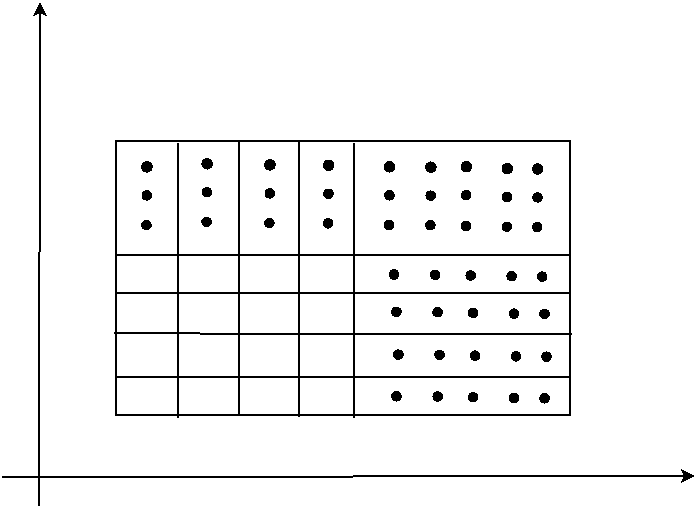
\includegraphics[scale=0.29]{./lattice.png} 
\end{center} 
\caption{Cuadrícula de $n\times m$}
\end{figure}
Este retículo se construye formalmente al dibujar lineas verticales y horizontales sobre el dentro del rectángulo $R$ en los puntos con coordenadas $(x_i, y_j)$, donde
\begin{equation}
x_i=a+ih,\,\,\,\text{para cada }i=0,1,2,\hdots,n\, \text{ y }\, y=a+jk,\,\,\,\text{para cada }j=0,1,2,\hdots,m
\end{equation}
Las rectas correspondientes a $x=x_i$ y $y=y_i$ son las lineas que forman la cuadricula y sus intersecciones son los puntos del retículo. Para cada punto interior del retículo se $(x_i,y_j)$, para $i=1,2,\hdots,n-1$ y $j=1,2,\hdots,m-1$, se puede utilizar una serie de Taylor en la variable $x$ alrededor del punto $x_i$ para generar una fórmula de diferencia centrada
\begin{equation}
\frac{\partial^2 u}{\partial x^2}(x_i,y_i)=\frac{u(x_{i+1},y_j)-2u(x_i,y_i)+u(x_{i-1},y_j)}{h^2}-\frac{h^2}{12}\frac{\partial^4 u}{\partial x^4}(\xi_i,y_j)
\end{equation}
donde $\xi_i \in (x_{i-1},x_{i+1})$. De igual manera se puede encontrar la serie de Taylor en la variable $y$ alrededor del punto $y_j$ para hallar la diferencia centrada
\begin{equation}
\frac{\partial^2 u}{\partial y^2}(x_i,y_i)=\frac{u(x_{i},y_{j+1})-2u(x_i,y_i)+u(x_{i},y_{j-1})}{k^2}-\frac{k^2}{12}\frac{\partial^4 u}{\partial y^4}(x_i,\eta_j)
\end{equation}
donde $\eta_i \in (y_{i-1},y_{i+1})$, sustituyendo estas fórmulas en las ecuación \ref{eq::Poisson} permite expresar la ecuación de Poisson en los puntos $(x_i,y_j)$ como
\begin{equation}
\begin{aligned}
&\frac{u(x_{i+1},y_j)-2u(x_i,y_i)+u(x_{i-1},y_j)}{h^2}+\frac{u(x_{i},y_{j+1})-2u(x_i,y_i)+u(x_{i},y_{j-1})}{k^2}\\
&=f(x_i,y_j)+\frac{h^2}{12}\frac{\partial^4 u}{\partial x^4}(\xi_i,y_j)+\frac{k^2}{12}\frac{\partial^4 u}{\partial y^4}(x_i,\eta_j)
\end{aligned}
\end{equation}
para cada $i=1,2,\hdots,n-1$ y $j=1,2,\hdots,m-1$. Las condiciones de contorno son
\begin{equation*}
u(x_0,y_j)=g(x_0,y_j)\,\, \text{ y } \,\, u(x_n,y_j)=g(x_n,y_j),\,\,\, \text{para cada }j=0,1,\hdots,m;
\end{equation*}
\begin{equation*}
u(x_i,y_0)=g(x_i,y_0)\,\, \text{ y } \,\, u(x_i,y_m)=g(x_i,y_m),\,\,\, \text{para cada }i=1,2,\hdots,n-1;
\end{equation*}
\subsection{Método de Diferencias Finitas}
En forma de ecuación de diferencias el Método de diferencias finitas es
\begin{equation}\label{eq::finite_difference}
2\Bigg[\Bigg(\frac{h}{k}\Bigg)^2 +1  \Bigg]w_{ij}-(w_{i+1,j}+w_{i-1,j})-\Bigg(\frac{h}{k}\Bigg)^2(w_{i,j+1}+w_{i,j-1})=-h^2 f(x_i,y_j)
\end{equation}
para cada $i=1,2,\hdots,n-1$ y $j=1,2,\hdots,m-1$, donde
\begin{equation}\label{eq:boundary_conditions}
\begin{aligned}
&w_{0j}=g(x_0,y_j)\,\,\text{y }\, w_{nj}=g(x_n,y_j),\,\,\, \text{para cada } j=0,1,\hdots,m;\\
&w_{i0}=g(x_i,y_0)\,\,\text{y }\, w_{im}=g(x_i,y_m),\,\,\, \text{para cada } i=1,2,\hdots,n-1
\end{aligned}
\end{equation}
donde $w_{ij}$ aproxima $u(x_i,y_j)$. Este método tiene un error de truncación del orden $O(h^2+k^2)$. La ecuación \ref{eq::finite_difference} involucra aproximaciones para $u(x,y)$ en los puntos
\begin{equation*}
(x_{i-1},y_{j}),\,\,\,(x_{i},y_{j}),\,\,\,(x_{i},y_{j-1}),\,\text{y}\,\,(x_{i},y_{j+1}).\,\,\,
\end{equation*}
Utilizando la información proveída por las condiciones de contorno \ref{eq:boundary_conditions} cuando el sistema definido por \ref{eq::finite_difference} lo permite, i.e. en los puntos adyacentes al contorno definido por la cuadrícula construida previamente(\ref{fig::mesh}).\\ Con esto se obtiene un sistema de ecuaciones con una matriz de incógnitas de dimensiones $(n-1)(m-1)\times(n-1)(m-1)$ donde las incognitas son las aproximaciones $w_{ij}$ para $u(x_i,y_j)$ en los puntos interiores del retículo(\ref{fig::mesh}).\\

El sistema lineal para las incógnitas $w_{ij}$ se puede representar más eficientemente para realizar operaciones matriciales si se realiza una re-etiquetación de de los puntos interiores del retículo, una recomendación para realizar este esquema de re-etiquetación puede hallarse en \cite{Varga} de la siguiente manera
\begin{equation}
P_l=(x_i,y_j), \,\,\, \text{y}\,\,\, w_l=w_{ij}
\end{equation}
donde
\begin{equation}\label{eq::relabeling_function}
l(i,j)=i+(m-1-j)(n-1)
\end{equation} 
para cada $i=1,2,\hdots,n-1$ y $j=1,2,\hdots,m-1$, con este esquema de etiquetan a los puntos interiores del retículo de izquierda a derecha y de arriba hacia abajo y con esto se asegura que el sistema lineal resultante para hallar $w_{ij}$ es una matriz con bandas de ancho máximo $2n-1$. Esta técnica fue utiliza para implementar este algoritmo en Python, ver algoritmos \ref{alg::funcL} y \ref{alg::finite_difference}.



\section{Algoritmo Método de Diferencias Finitas para ecuación de Poisson}
Para hallar un algoritmo que genere y resuelva el método de diferencias finitas para las ecuaciones parciales elípticas descrito en la sección anterior se usa el esquema de re-etiquetado expuesto anteriormente, con esto se asegura que se obtiene un sistema tri-diagonal por bloques. Para estos sistemas tri-diagonales por bloques es conveniente aplicar una generalización del algoritmo de Factorización de Crout \cite{Varga} para matrices tri-diagonales por bloques.\\
Otro algoritmo iterativo que se puede utilizar es el método de relajamiento SOR. Con esto se puede delinear una estrategia para construir un algoritmo para el método de diferencias finitas:
\begin{itemize}
\item Construir el sistema asociado a las aproximaciones $w_{ij}$ para $u(x_i,y_j)$, utilizando el esquema de etiquetado expuesto anteriormente.
\item Aplicar un método de resolución de sistemas lineales: Generalización de factorización de Crout, método iterativo SOR.
\item Resolver para $w_{ij}$
\end{itemize}

\subsection{Algoritmo diferencias finitas(sistema lineal)}
\subsubsection{Función de re-etiquetado l}
Se implementa la función $l$ para re-etiquetar el sistema de ecuaciones lineal
\begin{algorithm}[H]
\caption{Función L para re-etiquetar las variables del sistema lineal}\label{alg::funcL}
\begin{algorithmic}[H]
\Function L {$i, j, n, m$}
\State \Return $(i+1) + (m-1-(j+1)) \times (n-1) - 1$
\EndFunction
\end{algorithmic}
\end{algorithm}
\subsubsection{Sistema lineal asociado}
Con está función se crea el sistema asociado al método de diferencias finitas
\begin{algorithm}[H]
\caption{Finite Difference Linear System}\label{alg::finite_difference}
\begin{algorithmic}[H]
\Function{finite\_difference\_linear\_system}{$a,b,c,d,n,m,f,g$}
\State $h \gets (b-a)/n$
\State $k \gets (d-c)/n$
\State $x \gets \text{numpy.linspace}(a, b, n+1)$
\State $y \gets \text{numpy.linspace}(c, d, m+1)$
\State $W_{ij} \gets$ zeros $(((n-1)\times(m-1)),((n-1)\times(m-1)))$
\State $w \gets$ zeros $((n-1)\times(m-1))$
\For{$i \gets 0$ to $n-2$}
\For{$j \gets 0$ to $m-2$}
\State $W_{ij}[L(i,j,n,m), L(i,j,n,m)] \gets 2((h/k)^2 + 1)$
\If{$i \neq 0$ and $i \neq n-2$}
\State $W_{ij}[L(i,j,n,m), L(i+1,j,n,m)] \gets -1$
\State $W_{ij}[L(i,j,n,m), L(i-1,j,n,m)] \gets -1$
\Else
\If{$i = 0$}
\State $W_{ij}[L(i,j,n,m), L(i+1,j,n,m)] \gets -1$
\State $w[l(i,j,n,m)] \gets g(x[i], y[j+1], a, b, c, d)$
\EndIf
\If{$i = n-2$}
\State $W_{ij}[L(i,j,n,m), L(i-1,j,n,m)] \gets -1$
\State $w[L(i,j,n,m)] \gets g(x[i+2], y[j+1], a, b, c, d)$
\EndIf
\EndIf
\If{$j \neq 0$ and $j \neq m-2$}
\State $W_{ij}[L(i,j,n,m), L(i,j+1,n,m)] \gets -1$
\State $W_{ij}[L(i,j,n,m), L(i,j-1,n,m)] \gets -1$
\Else
\If{$j = 0$}
\State $W_{ij}[L(i,j,n,m), L(i,j+1,n,m)] \gets -(h/k)^2$
\State $w[L(i,j,n,m)] \gets g(x[i+1], y[j], a, b, c, d)$
\EndIf
\If{$j = m-2$}
\State $W_{ij}[L(i,j,n,m), L(i,j-1,n,m)] \gets -(h/k)^2$
\State $w[L(i,j,n,m)] \gets g(x[i+1], y[j+2], a, b, c, d)$
\EndIf
\EndIf
\State $w[L(i,j,n,m)] \gets -h^2f(x[i], y[j])+w[L(i,j,n,m)]$
\EndFor
\EndFor
\State \textbf{return} $W_{ij}, w$
\EndFunction
\end{algorithmic}
\end{algorithm}

\subsection{Algoritmo de Generalización Factorización de Crout para matrices tridiagonales por bloques}
Esta es la implementación de la generalización del algoritmo de factorización de Crout para matrices tri-diagonales por bloques, el algoritmo de factorización de Crout sólo es valido para matrices tri-diagonales y no para matrices tri-diagonales por bloques.
\begin{algorithm}[H]
\caption{Crout Generalization Algorithm for Tridiagonal Block Matrices}\label{alg::Crout}
\begin{algorithmic}[H]
\Require $A \in \mathbb{R}^{N \times N}$, $K \in \mathbb{R}^{N}$, $n \in \mathbb{N}$
\Ensure $sol \in \mathbb{R}^{N}$
\Function{Crout\_generalization}{$A, K, n$}
\State $N \gets \lfloor \frac{\operatorname{shape}(A)[1]}{n} \rfloor$
\State $W \gets []$
\State $B_1 \gets A_{1:n,1:n}$
\State $C_1 \gets A_{1:n,n:n+n}$
\State $W.append(\operatorname{inv}(B_1) \cdot C_1)$
\For{$i \gets 2$ to $N-1$}
\State $B_i \gets A_{(i-1)n:in,(i-1)n:in}$
\State $A_i \gets A_{(i-1)n:in,(i-2)n:(i-1)n}$
\State $C_i \gets A_{(i-1)n:in,in+1:n+(i-1)n}$
\State $W.append(\operatorname{inv}(B_i - A_i \cdot W_{i-2}) \cdot C_i)$
\EndFor
\State $B_N \gets A_{1:n,1:n}$
\State $K_1 \gets K_{1:n}$
\State $G_1 \gets \operatorname{inv}(B_1) \cdot K_1$
\State $G \gets []$
\State $G.append(G_1)$
\For{$i \gets 2$ to $N$}
\State $K_i \gets K_{(i-1)n:in}$
\State $B_i \gets A_{(i-1)n:in,(i-1)n:in}$
\State $A_i \gets A_{(i-1)n:in,(i-2)n:(i-1)n}$
\State $G.append(\operatorname{inv}(B_i - A_i \cdot W_{i-2}) \cdot (K_i - A_i \cdot G_{i-2}))$
\EndFor
\State $Z \gets G[:]$
\For{$i \gets N-2$ to $0$ step $-1$}
\State $Z_i \gets G_i - W_i \cdot Z_{i+1}$
\EndFor
\State $sol \gets \operatorname{concatenate}(Z)$
\State \textbf{return} $sol$
\EndFunction
\end{algorithmic}
\end{algorithm}
\subsection{Método iterativo SOR para resolver sistemas lineales}
\begin{algorithm}[H]
%\caption{Método iterativo SOR para resolver sistemas lineales}
\caption{Iterative SOR method for solving linear systems}\label{alg::SOR}
\begin{algorithmic}[H]
\Require{$A$ es una $n \times n$ matriz, $b$ es un vector de incógnitas de dimensión $n$, $x^{(0)}$ es una solución propuesta inicial, $\omega$ es el parámetro de relajamiento, $\epsilon$ es la tolerancia, and $max_{iter}$ es el número máximo de iteraciones.}
\Ensure{$x$ es una solución aproximada de $Ax = b$.}
\Function{SOR}{$A,b,\omega,\epsilon,\max_{iter},x^{(0)}$}
\State $k \gets 1$
\State $xo \gets x^{(0)}$
\State $tolerance\gets \textbf{True}$
\While{$k < max_{iter}$ and $\text{tolerance}$}
\For{$i = 1$ to $n$}
\State $s \gets \sum_{j=1}^{i-1} a_{ij}x_j + \sum_{j=i+1}^{n} a_{ij}xo_j$
\State $x_i \gets (1-\omega) xo_i + \frac{\omega}{a_{ii}} (b_i - s)$
\EndFor
\If{$||x - xo|| < \epsilon$}
\State $tolerance\gets \textbf{False}$
\EndIf
\State $k \gets k+1$
\State $xo=x$
\EndWhile
\If{$k = max_{iter}$}
\State \textbf{print} "Se ha alcanzado el número máximo de iteraciones"
\EndIf
\State \textbf{return} $x$
\EndFunction
\end{algorithmic}
\end{algorithm}

\subsection{Diferencia finitas usando generalización de factorización Crout}
\begin{algorithm}[H]
\caption{Algoritmo diferencias finitas usando generalización factorización de Crout}\label{alg::finite_diff_Crout}
Dado un problema con condiciones de frontera de la forma \ref{eq::Poisson}, definir
\begin{equation*}
a,b,c,d,n,m,f(x,y),g(x,y)
\end{equation*}
usando las funciones definidas en los algoritmos \ref{alg::finite_difference}, \ref{alg::Crout}
\begin{algorithmic}
%\State usar función definida en algoritmo 
\State $A, b\gets$ finite\_difference\_linear\_system$(a,b,c,d,n,m,f,g)$
%\State usar función definida en algoritmo 
\State $solution\gets $ Crout\_generalization(A,b,n-1)
\end{algorithmic}
\end{algorithm}
este algoritmo se ha implementado en Python, usando la librería Numpy. El repositorio se encuentra en \url{https://github.com/Julio-Medina/Finite_Difference_Method/tree/main/code}.
\subsection{Diferencia finitas usando método de relajamiento SOR}
\begin{algorithm}[H]
\caption{Algoritmo diferencias finitas usando generalización factorización de Crout}\label{alg::finite_diff_Crout}
Dado un problema con condiciones de frontera de la forma \ref{eq::Poisson}, definir
\begin{equation*}
a,b,c,d,n,m,f(x,y),g(x,y),\omega,\epsilon,x^{(0)}
\end{equation*}
usando las funciones definidas en los algoritmos \ref{alg::finite_difference}, \ref{alg::SOR}
\begin{algorithmic}
%\State usar función definida en algoritmo 
\State $A, b\gets$ finite\_difference\_linear\_system$(a,b,c,d,n,m,f,g)$
%\State usar función definida en algoritmo 
\State $solution\gets $ SOR($A,b,\omega,\epsilon,\max_{iter},x^{(0)}$)
\end{algorithmic}
\end{algorithm}
\subsection{Ejemplos}
Para ilustrar el funcionamiento del algoritmo no hay mejor forma que resolver algunos problemas con condiciones en la frontera.
\subsubsection{Ejemplo 1}
Resolver el siguiente problema 
\begin{equation}
\frac{\partial^2 u}{\partial x^2}(x,y)+\frac{\partial^2 u}{\partial y^2}(x,y)=0
\end{equation}
para cada $(x,y)$ en el conjunto $R=\{ (x,y)|\, 0<x<0.5,\, 0<y<0.5 \}$. Las condiciones de contorno  son 
\begin{equation*}
u(0,y)=0,\,u(x,0)=0,\, u(x,0.5)=200x,\, u(0.5,y)=200y,\,
\end{equation*}
Si $n=m=4$, la ecuación de diferencias finitas \ref{eq::finite_difference} da como resultado
\begin{equation}
4w_{i,j}-w_{i+1,j}-w_{i-1,j}-w_{i,j-1}-w_{i,j+1}=0
\end{equation}
para cada $i=1,2,3$ y $j=1,2,3$.\\
Por ejemplo cuando $i=1,j=1$ se obtiene
\begin{equation}\label{eq::finite_diff1}
4w_{1,1}-w_{2,1}-w_{0,1}-w_{1,0}-w_{1,2}=0
\end{equation}
pero $w_{1,0}=w_{0,1}=0$, usando la función de re-etiquetado \ref{eq::relabeling_function}  se obtiene
\begin{equation*}
l(1,1)=7,\,l(2,1)=8,\,l(1,2)=4
\end{equation*}
sustituyendo en \ref{eq::finite_diff1} y usando las condiciones de contorno se obtiene la ecuación
\begin{equation*}
4w_{7}-w_{8}-w_{4}=0
\end{equation*}
este proceso se repite para los indices restantes, dando como resultado $9$ ecuaciones lineales para las variables $w_1,w_2,w_3,w_4,w_5,w_7,w_8,w_9$. La matriz de coeficientes del sistema lineal obtenido al iterar a través de todos los indices es 
\begin{equation}\label{eq::block_tridiagonal_matrix_1}
A =
\begin{bmatrix}
4.0 & -1.0 & 0.0 & -1.0 & 0.0 & 0.0 & 0.0 & 0.0 & 0.0 \\
-1.0 & 4.0 & -1.0 & 0.0 & -1.0 & 0.0 & 0.0 & 0.0 & 0.0 \\
0.0 & -1.0 & 4.0 & 0.0 & 0.0 & -1.0 & 0.0 & 0.0 & 0.0 \\
-1.0 & 0.0 & 0.0 & 4.0 & -1.0 & 0.0 & -1.0 & 0.0 & 0.0 \\
0.0 & -1.0 & 0.0 & -1.0 & 4.0 & -1.0 & 0.0 & -1.0 & 0.0 \\
0.0 & 0.0 & -1.0 & 0.0 & -1.0 & 4.0 & 0.0 & 0.0 & -1.0 \\
0.0 & 0.0 & 0.0 & -1.0 & 0.0 & 0.0 & 4.0 & -1.0 & 0.0 \\
0.0 & 0.0 & 0.0 & 0.0 & -1.0 & 0.0 & -1.0 & 4.0 & -1.0 \\
0.0 & 0.0 & 0.0 & 0.0 & 0.0 & -1.0 & 0.0 & -1.0 & 4.0 \\
\end{bmatrix}
\end{equation}
y el vector constante es 
\begin{equation*}
b =
\begin{bmatrix}
25.0 \\
50.0 \\
150.0 \\
0.0 \\
0.0 \\
50.0 \\
0.0 \\
0.0 \\
25.0 \\
\end{bmatrix}
\end{equation*}
Es importante notar que la matriz resultante \ref{eq::block_tridiagonal_matrix_1} es una matriz tri-diagonal por bloques con cada bloque de dimensión $3\times 3$. Con esto se puede resolver el sistema
\begin{equation}
Aw=b
\end{equation}
donde se obtiene
\begin{equation}
\begin{bmatrix}
w_1 \\
w_2 \\
w_3 \\
w_4 \\
w_5 \\
w_6 \\
w_7 \\
w_8 \\
w_9 \\
\end{bmatrix}=
\begin{bmatrix}
18.75 \\
37.5 \\
56.25 \\
12.5 \\
25 \\
37.5 \\
6.25 \\
12.5 \\
18.75 \\
\end{bmatrix}
\end{equation}

\subsubsection{Ejemplo 2}
Resolver el siguiente problema 
\begin{equation}
\frac{\partial^2 u}{\partial x^2}(x,y)+\frac{\partial^2 u}{\partial y^2}(x,y)=x-y
\end{equation}
para cada $(x,y)$ en el conjunto $R=\{ (x,y)|\, 0<x<12,\, 0<y<12 \}$. Las condiciones de contorno  son 
\begin{equation*}
u(0,y)=0,\,u(x,0)=0,\, u(x,2)=10x^2,\, u(2,y)=200y
\end{equation*}
Si $n=6,\,\,m=4$, la ecuación de diferencias finitas \ref{eq::finite_difference} da como resultado
\begin{equation}
4w_{i,j}-w_{i+1,j}-w_{i-1,j}-w_{i,j-1}-w_{i,j+1}=-4(x_i-y_i)
\end{equation}
La matriz de coeficientes asociada $A$ es 
\begin{equation}
\begin{bmatrix}
 4.0 & -1.0 &  0.0 &  0.0 &  0.0 & -1.0 &  0.0 &  0.0 &  0.0 &  0.0 &  0.0 &  0.0 &  0.0 &  0.0 &  0.0 \\
-1.0 &  4.0 & -1.0 &  0.0 &  0.0 &  0.0 & -1.0 &  0.0 &  0.0 &  0.0 &  0.0 &  0.0 &  0.0 &  0.0 &  0.0 \\
 0.0 & -1.0 &  4.0 & -1.0 &  0.0 &  0.0 &  0.0 & -1.0 &  0.0 &  0.0 &  0.0 &  0.0 &  0.0 &  0.0 &  0.0 \\
 0.0 &  0.0 & -1.0 &  4.0 & -1.0 &  0.0 &  0.0 &  0.0 & -1.0 &  0.0 &  0.0 &  0.0 &  0.0 &  0.0 &  0.0 \\
 0.0 &  0.0 &  0.0 & -1.0 &  4.0 &  0.0 &  0.0 &  0.0 &  0.0 & -1.0 &  0.0 &  0.0 &  0.0 &  0.0 &  0.0 \\
-1.0 &  0.0 &  0.0 &  0.0 &  0.0 &  4.0 & -1.0 &  0.0 &  0.0 &  0.0 & -1.0 &  0.0 &  0.0 &  0.0 &  0.0 \\
 0.0 & -1.0 &  0.0 &  0.0 &  0.0 & -1.0 &  4.0 & -1.0 &  0.0 &  0.0 &  0.0 & -1.0 &  0.0 &  0.0 &  0.0 \\
 0.0 &  0.0 & -1.0 &  0.0 &  0.0 &  0.0 & -1.0 &  4.0 & -1.0 &  0.0 &  0.0 &  0.0 & -1.0 &  0.0 &  0.0 \\
 0.0 &  0.0 &  0.0 & -1.0 &  0.0 &  0.0 &  0.0 & -1.0 &  4.0 & -1.0 &  0.0 &  0.0 &  0.0 & -1.0 &  0.0 \\
 0.0 &  0.0 &  0.0 &  0.0 & -1.0 &  0.0 &  0.0 &  0.0 & -1.0 &  4.0 &  0.0 &  0.0 &  0.0 &  0.0 & -1.0 \\
 0.0 &  0.0 &  0.0 &  0.0 &  0.0 & -1.0 &  0.0 &  0.0 &  0.0 &  0.0 &  4.0 & -1.0 &  0.0 &  0.0 &  0.0 \\
 0.0 &  0.0 &  0.0 &  0.0 &  0.0 &  0.0 & -1.0 &  0.0 &  0.0 &  0.0 & -1.0 &  4.0 & -1.0 &  0.0 &  0.0 \\
 0.0 &  0.0 &  0.0 &  0.0 &  0.0 &  0.0 &  0.0 & -1.0 &  0.0 &  0.0 &  0.0 & -1.0 &  4.0 & -1.0 &  0.0 \\
 0.0 &  0.0 &  0.0 &  0.0 &  0.0 &  0.0 &  0.0 &  0.0 & -1.0 &  0.0 &  0.0 &  0.0 & -1.0 &  4.0 & -1.0 \\
 0.0 &  0.0 &  0.0 &  0.0 &  0.0 &  0.0 &  0.0 &  0.0 &  0.0 & -1.0 &  0.0 &  0.0 &  0.0 & -1.0 &  4.0 \\
\end{bmatrix}
\end{equation}
y el vector constante es 
\begin{equation*}
b =
\begin{bmatrix}
 64.0 \\
 176.0 \\
 368.0 \\
 640.0 \\
2792.0 \\
  12.0 \\
   4.0 \\
  -4.0 \\
 -12.0 \\
1180.0 \\
   0.0 \\
  -8.0 \\
 -16.0 \\
 -24.0 \\
 568.0 \\
\end{bmatrix}
\end{equation*}
Es importante notar que la matriz resultante \ref{eq::block_tridiagonal_matrix_1} es una matriz tri-diagonal por bloques con cada bloque de dimensión $5\times 5$. Con esto se puede resolver el sistema
\begin{equation}
Aw=b
\end{equation}
donde se obtiene
\begin{equation}
\begin{bmatrix}
w_1 \\
w_2 \\
w_3 \\
w_4 \\
w_5 \\
w_6 \\
w_7 \\
w_8 \\
w_9 \\
w_{10} \\
w_{11} \\
w_{12} \\
w_{13} \\
w_{14} \\
w_{15} \\
\end{bmatrix}=
\begin{bmatrix}
  85.391560 \\
 201.165141 \\
 376.447717 \\
 640.071973 \\
1053.341871 \\
  76.401101 \\
 166.821284 \\
 296.553756 \\
 490.498303 \\
 781.295511 \\
  41.391560 \\
  89.165141 \\
 156.447717 \\
 256.071973 \\
 401.341871 \\
\end{bmatrix}
\end{equation}
\subsubsection{Ejemplo 3}
Resolver el siguiente problema 
\begin{equation}
\frac{\partial^2 u}{\partial x^2}(x,y)+\frac{\partial^2 u}{\partial y^2}(x,y)=x e^{y}
\end{equation}
para cada $(x,y)$ en el conjunto $R=\{ (x,y)|\, 0<x<2,\, 0<y<1 \}$. Las condiciones de contorno  son 
\begin{equation*}
u(0,y)=0,\,u(x,0)=x,\, u(x,1)=ex,\, u(2,y)=2e^y
\end{equation*}
Con $n=6,\,\,m=5$, comparar las aproximaciones con la solución analítica $u(x,y)=x e^y$



\begin{thebibliography}{99}
%% La bibliografía se ordena en orden alfabético respecto al apellido del 
%% autor o autor principal
%% cada entrada tiene su formatado dependiendo si es libro, artículo,
%% tesis, contenido en la web, etc


\bibitem{Burden} Richard L. Burden, J. Douglas Faires \textit{Numerical Analysis}, (Ninth Edition). Brooks/Cole, Cengage Learning. 978-0-538-73351-9

\bibitem{Varga} Richard S. Varga. \textit{Matrix Iterative Analysis}. Second Edition. Springer. DOI 10.1007/978-3-642-05156-2

%\bibitem{Feynman} 
%\bibitem{Hopfield} J.J. Hopfield. \textit{Neural Networks and physical systems with emergent collective computational abilities}. \url{https://doi.org/10.1073/pnas.79.8.2554}


%\bibitem{McCulloch} Warren S. McChulloch, Walter H. Pitts. \textit{A LOGICAL CALCULUS OF THE IDEAS IMMANENT IN NERVOUS ACTIVITY}. \url{http://www.cse.chalmers.se/~coquand/AUTOMATA/mcp.pdf}



\end{thebibliography}
\end{document}

